\documentclass{article}

\RequirePackage[top=1.25in,bottom=1.25in,left=1.25in,right=1.25in]{geometry}
\RequirePackage[labelfont=bf]{caption}
\RequirePackage{amsmath,amsfonts,verbatim,amsthm,tabularx,graphicx,amssymb,subfigure,color,enumitem,fancyhdr,epsfig,commath}
\RequirePackage[colorlinks=true,linkcolor=red,pagecolor=black,citecolor=red]{hyperref}
\RequirePackage[all]{hypcap}

\RequirePackage{minted}
\renewcommand{\theFancyVerbLine}{%
  \sffamily\textcolor[rgb]{0.5,0.5,0.5}{\normalsize\arabic{FancyVerbLine}}}

\newcommand{\given}{\, |\,}

\setlength{\captionmargin}{0.5in}


\begin{document}

    \begin{center}
        \Large
        Simple and Extensible Probabilistic Programming\\
        \vspace{0.1in}
        \normalsize
        Matthew Johnson\\
        Eyal Dechter\\
        \vspace{0.1in}
        \footnotesize
        Revised \today
    \end{center}

    \tableofcontents

    \newpage

    \begin{abstract}
        We describe the design and implementation of a probabilistic
        programming system in MIT Scheme. The system can perform generic
        probabilistic inference over any probability distribution specified as
        a Scheme program which generates random values. That is, given a Scheme
        program specifying a generative (forward) probability model and
        (optionally) some data on which to condition the model, our system
        provides mechanisms for providing random samples from the conditional
        model and thus for answering probabilistic inference queries with
        greatly reduced programmer effort.

        There are many probabilistic programming languages. Our system is most
        comparable to MIT Church: both allow simple specification of generative
        models in Scheme and provide generic inference through the same
        algorithm, an application of Metropolis-Hastings Markov-Chain Monte
        Carlo to the program's random choices. However, our system has several
        advantages:
        \begin{itemize}
            \item Our system is very small. By leveraging first-class
                continuations, we implement generic inference in about one
                hundred lines instead of thousands.
            \item Our system does not require an interpreter within Scheme;
                user programs are standard Scheme programs. One salient benefit
                is that all our code, including all user programs, can be
                compiled to machine code with the MIT Scheme compiler. Another
                is that it is very easy to set up and use.
            \item Our system has a generically-extensible design so that
                algorithms to exploit special probabilistic structure can be
                added, providing the potential to reduce or eliminate reliance
                on the inefficient MH algorithm in tractable cases.
        \end{itemize}

        In this document we briefly overview the goals of probabilistic
        programming and explain the generic Metropolis-Hastings algorithm as
        applied to sampling over probabilistic programs. We also detail our
        base system's interface and implementation, and we outline its design
        for generic extensibility along with examples of two in-progress
        extensions. Finally, we provide complete source listings and some
        example runs.

        Our source code is available at \url{https://github.com/mattjj/probprog}.
    \end{abstract}

\section{Example uses}
See Listing~\ref{listing:demo1} and Listing~\ref{listing:demo2}.

\begin{listing}[hp]
\begin{minted}[linenos,mathescape,numbersep=5pt,gobble=0,frame=lines,fontsize=\small,framesep=2mm]{scheme}
(load "load")

;;;; set up a simple discrete test

(define (test1)
  (let ((x (discrete '(0 1)))
        (y (discrete '(0 1)))
        (z (discrete '(0 1))))
    (let ((sum (+ x y z)))
      (emit (or (= sum 0)
                (= sum 2))
            #t)
      (list x y z))))

;;;; inspect a few samples

(test1)

;Value 2: (1 1 0)

(test1)

;Value 3: (0 1 1)

(test1)

;Value 4: (0 0 0)

;;;; construct a stream of samples
;; no burn-in and 5 MH steps between samples

(define ss (sample-stream test1 0 5))

(stream-head ss 10)

;Value: ((0 0 0) (0 0 0) (0 0 0) (1 1 0) (1 1 0) (1 1 0) (0 1 1) (0 1 1) (1 0 1) (1 1 0))

;;;; estimate the probability all are zero

(define (all-zero? s)
  (if (= (reduce + 0 s) 0)
    1
    0))

(estimate-mean (stream-map all-zero? ss) 2000)

;Value: 103/400

(estimate-mean (stream-map all-zero? ss) 4000)

;Value: 1/4

;;;; the true probability is 1/4
\end{minted}
\caption{A simple discrete inference problem.}
\label{listing:demo1}
\end{listing}

\begin{listing}[hp]
\begin{minted}[linenos,mathescape,numbersep=5pt,gobble=0,frame=lines,fontsize=\small,framesep=2mm]{scheme}
(load "load")

;;;; set up a simple Gaussian test

(define (test3)
  (let ((x (gaussian 0 1))
        (y (gaussian 0 4)))
    (emit (+ x y) 3 (likelihood:additive-gaussian 0 1))
    y))

;;;; inspect a few samples

(test3)

;Value: 2.627738902766393

(test3)

;Value: 1.4713636283192144

(test3)

;Value: 3.650811672098934

(test3)

;Value: 2.508292233153293

;;;; construct a stream of samples from the Markov chain
;; 5000 steps for burn-in and 25 MH steps between samples

(define ss (sample-stream test3 5000 25))

(stream-head ss 5)

;Value: (2.362360472725903 2.457989361328277 .9664606900582463 2.245335036134793 2.241072726252283)

;;;; estimate the mean

(estimate-mean ss 2000)

;Value: 2.0789872746395206

(estimate-mean ss 3000)

;Value: 2.0538287789004213

;;;; the true posterior mean is 2
\end{minted}
\caption{A simple Gaussian inference problem.}
\label{listing:demo2}
\end{listing}


\section{Overview of probabilistic programming}
The goal of probabilistic programming is to enable the user to perform
probabilistic inference by writing down a probability distribution in a purely
declarative fashion. Thus, probabilistic programming is to probabilistic
inference what logic programming is to first order logic: instead of specifying
what the computer should do, the user specifies constraints on the computer's
output, leaving hidden the mechanism and algorithm by which the computer finds
the answer. In logic programming, the user writes down a set of logical
statements and can then ask various queries of the system. Similarly, in
probabilistic programming, the goal is to be able to accommodate various
queries from the declared probability distribution, such as sampling from the
distribution and reporting statistics related to the distribution.  

How does one declare a probability distribution? Various alternatives exist in
the literature. One class of probabilistic programming languages extends logic
programming to accommodate probabilities; these include Markov
Logic~\cite{richardson2006markov} and Independent Choice
Logic~\cite{poole1997independent}. Another class of languages captures directly
the structure of a ``graphical model," a representation of probability
distributions as a graph in which component distributions represent nodes and
edges represent dependencies; for an exmple of this, see
BUGS~\cite{lunn2000winbugs} or JAGS~\cite{plummer2003jags}. 

Sampling procedures or ``generative processes" are an alternative way to
represent probability distributions simply as the output of a stochastic
sampling procedure, i.e., a computer program with random primitives. A large
number of languages, including the one we present here, use functional or
imperative languages with stochastic primitives as the backbone of a
probabilistic programming language. In general, one also needs to be able to
condition on one or more of the variables in
the program taking on a specific value. These languages usually contain explicit
constructs that enable such conditioning. As examples of these languages see
BLOG~\cite{milch20071} or Church~\cite{goodman2012church}.

This last approach is by far the most flexible of the three presented above. It
accommodates, after all, the distribution over the output of any program that one
could write in, for example, scheme. How can we perform inference for arbitrary
programs? A special case of this problem, after all, is to observe the output of
any deterministic scheme function and return a satistfying set of inputs.

In the next two sections, we will describe the Metropolis-Hastings algorithm
(known as MH) which can, in principle, be used to perform inference over
arbitrary program traces. However, MH is a slow and approximate algorithm, with
no guarantee of accuracy for any finite amount of running time. Specialized
inference algorithms for particular families of probability distributions exist
throughout the statistical inference literature. Discrete graphical models over
large numbers of variables can be solved exactly and efficiently if the model
has low ``tree-width." Continuous probability distribution whose gradients we can
evaluate can be sampled from efficiently with Hamiltonian Monte Carlo~\cite{duane1987hybrid}.
And collections of probability distributions that are ``conjugate" to another
can often be queried very quickly; such conjugate pairs of distributions exist
for any distribution in the ``exponential family" distributions.

One of the goals of this project is to show how an MH based probabilistic
program can be extended to use specialized inference algorithms. 

\section{Rejection sampling}
We briefly note that a simple universal inference algorithm exists that is
simpler than the MH algorithm we describe in the next section: rejection sampling.
In rejection sampling, we can get unbiased samples from the posterior
distribution of any of the random variables in the program by sampling program
traces from the prior and keeping only the traces that agree with the
\verb+emit+ call. Although the rejection sampling algorithm is
guaranteed to give exact samples from the posterior, it is not practical for
all but the simplest of probability  distributions because in most cases the
probability of the event on which we are conditioning is vanishingly small. In
effect, trying to perform inference in a probabilistic program by rejection
sampling would be akin to trying to find a solution to an AMB problem by making
random nondeterministic choices and hoping that you hit a valid solution.

\section{The Metropolis-Hastings algorithm}

The Metropolis-Hastings Algorithm is a general purpose algorithm for sampling $x
\sim p(x)$ in cases where we only have direct access to $p^*(x) \propto
p(x)$. MH works by constructing a Markov chain over the state space $X$ whose
stationary distribution is $p(x)$. Thus, to specify the algorithm, we need to
specify the transition operator $T(x'\,|\,x)$, i.e. the probability of choosing
location $x'$ as the next state given that the current state is $x$. 

To do this, we need to define a proposal distribution $Q(x' \, | \, x)$. This
distribution is up to the user, and is often a relatively local transition. For
example, in continuous domains, $Q(x' \, | \, x) \sim N(x-x', \sigma)$ is a common
choice. 

Once we have proposed a transition to $x'$, we decide whether to accept that
proposal based on the relative value of $p^*(x) Q(x' \,| \, x)$ vs. $p^*(x') Q(x
\,| \, x')$. Formally, the probability of transitioning from $x$ to $x'$ is
given by  

\begin{align}
T(x'\, |\, x) =& Q(x' \, |\, x)\min \left \{1, 
                    \frac{p^*(x') Q(x \, |\, x')} 
                    {p^*(x) Q(x' \, |\, x)} \right \}.
                    \label{eq:MHTransitionProb}
\end{align}

It is easy to show that, under mild conditions, this transition rule results in
a Markov chain whose stationary distribution is $p(x)$.

\section{The structure of a probabilistic program}

The probabilistic programming language we designed is written as regular scheme
code except for one special construct, \verb+emit+.  Although it is itself just a
regular scheme function, semantically, \verb+(emit x x-val)+ conditions the
probability distribution defined by the rest of the code on the fact that
variable \verb+x+ is equal to \verb+x-val+. \verb+emit+ takes an optional
argument that specifies what kind if any observation noise should be associated
with the observation of this variable.

An example program and conditions on the output of the sum of two Gaussian
variable being equal to ten might look like

\begin{minted}[linenos,mathescape,numbersep=5pt,gobble=0,frame=lines,fontsize=\small,framesep=2mm]{scheme}
(define (sum-of-gaussians)
    (let ( (x (gaussian 7 2))
           (y (gaussian 5 3)))
        (emit (+ x y) 10 observation-likelihood)))
\end{minted}

This elucidates the general structure of a probabilistic program: we write down
a regular scheme function that calls some stochastic primitives (that are either
user-defined or provided as a base library). At the end of the program, we can
condition on any variable or function of variables being equal to some value. 

\section{The Metropolis-Hastings algorithm for program traces}
Every time we run a program that evaluates stochastic functions, the set of
random choices that are made, which we will call the \emph{ptrace}, corresponds
to a state in the domain of the distribution defined by the program. To
transition to another state, we need to change those random choices in some
manner. Here we propose a specific proposal distribution over ptraces and show
how to calculate the acceptance probability defined in the previous section. 

We define a proposal distribution $Q_{ptrace}(\bar{x}'\given \bar{x} )$ by
choosing a choice point from $\bar{x}$ uniformly at random and running the program
from that point forward. Suppose we choose to propose a new $i$th choice point.
Let $\bar{x}_{before}$ specify the choices before the $i$th choice and let
$\bar{x}_{after}$ and $\bar{x}'_{after}$ refer to the choices made after the
$i$th choice in the original ptrace and the proposed one, respectively. Then
\begin{align}
Q(\bar{x}' \given \bar{x}) =& \frac{1}{\text{length}(\bar{x})} 
                            q(x'_i \given x_i) p(\bar{x}'_{after} \given
                            \bar{x}_{before}, x'_i)
                            p(y | \bar{x}').
\end{align}

The target distribution we want to sample from 
\begin{align}
p(\bar{x} \given y) \propto & p(y \given \bar{x}) p(\bar(x))\\
                    =& p(\bar{x}_{before}) p(x_i \given \bar{x}_{before})
                    p(\bar{x}_{after} \given \bar{x}_{before}, x_i)
                    p(y|\bar{x}).
\end{align}

So the acceptance ratio in Equation~\ref{eq:MHTransitionProb} is

\begin{align}
\frac{p(\bar{x}'_{before}) p(x'_i \given \bar{x}'_{before})
                    p(\bar{x}'_{after} \given \bar{x}'_{before}, x'_i)
                   p(y|\bar{x}')}
                   {p(\bar{x}_{before}) p(x_i \given \bar{x}_{before})
                    p(\bar{x}_{after} \given \bar{x}_{before}, x_i)
                    p(y|\bar{x})}\\
\frac{\frac{1}{\text{length}(\bar{x'})} 
                           q(x_i \given x'_i) p(\bar{x}_{after} \given \bar{x}_{before}, x_i)
                        }{\frac{1}{\text{length}(\bar{x})} 
                           q(x'_i \given x_i) p(\bar{x}'_{after} \given
                           \bar{x}'_{before}, x'_i)}\\
= \frac{p(x'_i \given \bar{x}'_{before})
        p(y|\bar{x}')}
{p(x_i \given \bar{x}_{before})
 p(y|\bar{x})}
\frac{\text{length}(\bar{x})
    q(x_i \given x'_i) }
    {\text{length}(\bar{x}') 
    q(x'_i \given x_i)}\\
\end{align}

In words, then, every transition involves picking a random point on the trace,
rolling it forward to the emit statement, and then comparing how well the new
trace fits the data to how well the old data fits the data. If we follow the MH
acceptance rule when choosing whether to accept or reject the new state, then
the stationary distribution of the Markov chain induced by these transitions
tends towards the target distribution.  A schematic of this process, within a
concrete example, is shown in Figure~\ref{fig:ptrace}.  


\begin{figure}
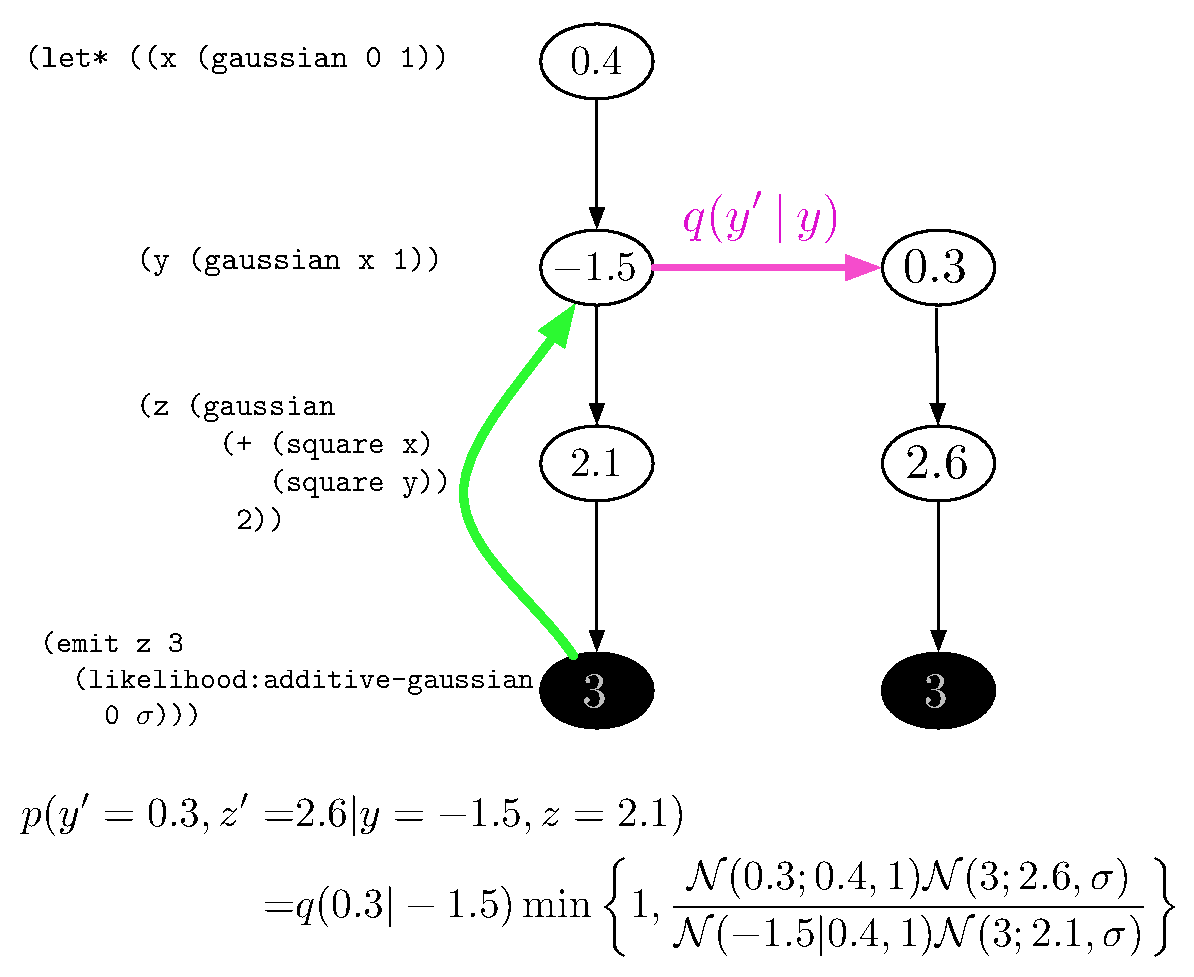
\includegraphics[width=\textwidth]{figures/ptrace.pdf}
\caption{The Metropolis-Hastings algorithm over program traces records the
stochastic choice points in the ptrace (i.e. the probabilistic trace). When it
hits an emit declaration, it chooses random choice point, proposes a new
value for that choice from $q(\cdot | \cdot)$ and rolls the program forward from
that point. It accepts or rejects the new trace according the
Metropolis-Hastings acceptance ratio.} \label{fig:ptrace}
\end{figure}



\section{System specifications}
\subsection{Overview}

In our system, probabilistic programs are standard Scheme procedures which call
our special random sampling procedures and emit procedure. These special
procedures communicate across calls by accessing and updating the global state
required for executing the Metropolis-Hastings algorithm over program traces.

The most significant global state is a representation of the sequence of random
choices made by the probabilistic program; each time a random sampling function
is called, a representation of the random choice is added to the global
sequence of choices. The representation of each choice includes a saved
continuation for that point in the probabilistic program so that choices can be
revisited and new values can be tried.

When the emit call is reached it acts as a barrier: the execution thread does
not proceed beyond the call to emit until some number of Metropolis-Hastings
iterations have been performed on the execution trace before the emit.  Each
Metropolis-Hastings iteration proceeds from the call to emit, and consists of
selecting a random choice to revisit, proposing a new value for that choice,
and executing the program forward until emit is again reached. With two
execution traces essentially waiting at the call to emit, one of the two
execution traces is selected with a probability determined by the Metropolis
acceptance probability.

For the purposes of this document, we only allow probabilistic programs to have
a single emit statement per execution path. It is relatively straightforward to
define a semantics which allows multiple ``partial'' emit statements, perhaps
with ID tags to associate emitted values with bindings in some
conditioning-data environment

Note that the extensible version of our systemis slightly different than the
system described here. The main difference is that in the extensible system
random values are boxed so that extra information can be tracked. For a
description of the extensible system, see Section~\ref{sec:foo}.

The following subsections describe the basic system and its implementation.
First, we describe the highest-level interfaces for user code. Next, we
describe the interfaces for extending the system with new random samplers, MH
proposal distributions, and emission likelihood functions. Finally we highlight
some parts of the back-end MH controller.

\subsection{User interface for writing probabilistic programs}

\subsubsection{Generating random values}
\begin{itemize}
    \item[] \texttt{(gaussian \emph{mean} \emph{var} [\emph{proposal-fn}])}\\
        Generates a Gaussian random variable with given mean (a number) and
        variance (a positive number). The optional argument
        \texttt{proposal-fn} defaults to additive Gaussian proposals with mean
        0 and variance one quarter of the sampling distribution's variance,
          i.e.~the value of \texttt{(proposals:additive-gaussian 0 (/ var 4))}.
    \item[] \texttt{(categorical \emph{items} [\emph{weights}] [\emph{proposal-fn}])}\\
        Generates a random sample from the list \texttt{\emph{items}}. If the
        optional argument \texttt{weights} is provided, it should be a list of
        numbers specifying (up to proportionality) the probabilities for the
        corresponding entries of \texttt{items} to be selected. The optional
        argument \texttt{proposal-fn} defaults to sampling from the prior.
\end{itemize}

\subsubsection{Conditioning on data}
\begin{itemize}
    \item[] \texttt{(emit \emph{random-value} \emph{observed-value} [\emph{likelihood-fn}])}\\
        A call to emit effectively conditions on \texttt{random-value} taking
        on the value of \texttt{observed-value} in the sense that after the
        call to \texttt{emit} random assignments will be sampled according to
        the conditional (posterior) distribution implied by conditioning the
        generative process (prior) on the observation implied by the arguments
        to \texttt{emit}. The optional argument \texttt{likelihod-fn} defaults
        to \texttt{likelihood:exact}. For continuous quantities, it is
        necessary to use a likelihood function that gives ``partial credit'',
        such as \texttt{likelihood:additive-gaussian}.
\end{itemize}

\subsubsection{Running samplers}
A probabilistic program can be run as any other kind of Scheme procedure.
However, we provide mechanisms for encapsulating probabilistic programs so that
they can be managed more effectively and so that results from probabilistic
programs can be used in other probabilistic programs. All the following
procedures encapsulate the running of a probabilistic program in the sense that
they dynamically rebind the global state variables used in the MH algorithm via
a \texttt{fluid-let}.

\begin{itemize}
    \item[] \texttt{(run \emph{pthunk} \emph{num-iterations})}\\
        Runs the zero-arity probabilistic program \texttt{pthunk} for
        \texttt{num-iterations} Metropolis-Hastings steps before returning the
        value. This procedure also has the side effect of adding
        \texttt{pthunk}'s running MH state to a global hash table so that it
        can be resumed by a call to \texttt{resume}. Repeated calls to
        \texttt{run} will simply clobber the saved state and effectively
        restart the sampler.
    \item[] \texttt{(resume \emph{pthunk} \emph{num-iterations})}\\
        Given a zero-arity probabilistic program \texttt{pthunk} on which
        \texttt{run} has already been called, runs \texttt{pthunk} for
        \texttt{num-iterations} Metropolis-Hastings steps before returning the
        value, but it resumes the MH Markov Chain from its most recent state.
        The ability to resume the sampler allows us to re-use the ``burn-in''
        time spent in which typical samplers wander to areas of high
        probability in the posterior from their random initializations.
    \item[] \texttt{(sample-stream \emph{pthunk} \emph{burnin-iter} \emph{iter-between-samples})}\\
        Given a zero-arity probabilistic program \texttt{pthunk}, create a
        (lazy, memoized) Scheme stream of samples from \texttt{pthunk} by first
        running it for \texttt{burnin-iter} iterations and then adding a sample
        to the stream every \texttt{iter-between-samples} iterations.

        For example, we might attain incrementally better estimates of the mean
        of \texttt{pthunk} by the following sequence of calls:

        \texttt{(define ss (sample-stream my-pthunk 5000 50))}\\
        \texttt{(/ (stream-head-fold-left + 0 ss 1000) 1000.)}\\
        \texttt{(/ (stream-head-fold-left + 0 ss 2000) 2000.)}\\
        \texttt{(/ (stream-head-fold-left + 0 ss 3000) 3000.)}
    \item[] \texttt{(estimate-mean \emph{sample-stream} \emph{num-samples})}
        \texttt{(estimate-variance \emph{sample-stream} \emph{num-samples})}
        Convenience functions for estimating averages of statistics of samples.
\end{itemize}

Here are possible implementations of \texttt{run} and \texttt{resume}:

\begin{listing}[H]
\begin{minted}[linenos,mathescape,numbersep=5pt,gobble=0,frame=lines,fontsize=\small,framesep=2mm]{scheme}
(define (run thunk niter)
(fluid-let (...) ;; binding global state
  (call-with-current-continuation
    (lambda (k)
      (fluid-let ((*top-level* k))
                 (let ((val (thunk)))
                   (eq-put! thunk 'last-ptrace *current-ptrace*)
                   (eq-put! thunk 'total-iterations *niter-done*)
                   (*top-level* (random-value:force val))))))))

(define (resume thunk niter)
  (call-with-current-continuation
    (lambda (k)
      (within-continuation
        (ptrace:emit-continuation (eq-get thunk 'last-ptrace))
        (lambda () (set! *niter-left* niter) (set! *top-level* k) #!unspecific)))))
\end{minted}
\caption{Implementations of \texttt{run} and \texttt{resume}.}
\label{listing:run-and-resume}
\end{listing}

Here are possible implementations of \texttt{estimate-mean} and \texttt{estimate-variance}:

\begin{listing}[H]
    \begin{minted}[linenos,mathescape,numbersep=5pt,gobble=0,frame=lines,fontsize=\small,framesep=2mm]{scheme}
(define (estimate-mean sample-stream nsamples)
  (/ (stream-head-fold-left + 0 sample-stream nsamples) nsamples))

(define (estimate-variance sample-stream nsamples)
  (- (estimate-mean (stream-map square sample-stream) nsamples)
     (square (estimate-mean sample-stream nsamples))))
    \end{minted}
    \caption{Implementations of \texttt{estimate-mean} and \texttt{estimate-varnace}.}
\end{listing}

\subsection{Interface for adding samplers and proposers}

\subsubsection{Sampling random values}
\begin{itemize}
    \item[] \texttt{(sample \emph{sampler-fn} \emph{likelihood-fn} \emph{proposer-fn})}\\
        \texttt{sampler-fn} is a function of no arguments that produces random sample values.\\
        \texttt{likelihood-fn} is a function that takes one argument of the
        same type as the output of \texttt{sampler-fn} and returns a log
        likelihood value (value of the log density with respect to Lebesgue
        measure) for its argument value.\\
        \texttt{proposer-fn} is a procedure that takes one argument of the same
        type as the output of \texttt{sampler-fn} and returns a new random
        value of the same type and also sets the global variables
        \texttt{*forward-score*} and \texttt{*backward-score*} appropriately.

        The \texttt{sample} function does the choice/continuation bookkeeping
        necessary for the MH back-end.
\end{itemize}

For example, the procedure \texttt{gaussian} can be implemented using \texttt{sample}:

\begin{listing}[H]
\begin{minted}[linenos,mathescape,numbersep=5pt,gobble=0,frame=lines,fontsize=\small,framesep=2mm]{scheme}
(load "randutil")
(define (gaussian mean var #!optional proposer)
  (if (default-object? proposer)
    (set! proposer (proposals:additive-gaussian 0 (/ var 4))))

  (let ((params (gaussian:make-params mean var)))
    (sample
      (lambda () (random-value:new 'gaussian (gaussian:rvs params)))
      (lambda (rv) (gaussian:log-likelihood (random-value:val rv) params))
      proposer)))
\end{minted}
\caption{An implementation of \texttt{gaussian}.}
\label{listing:gaussian}
\end{listing}

Proposal functions take a random value as an argument and propose a new one.
They also set global state. Here is an example:

\begin{listing}[H]
\begin{minted}[linenos,mathescape,numbersep=5pt,gobble=0,frame=lines,fontsize=\small,framesep=2mm]{scheme}
(define ((proposals:additive-gaussian mean var) rv)
  (let* ((params (gaussian:make-params mean var))
         (nudge (gaussian:rvs params))
         (proposal-score (gaussian:log-likelihood nudge params))
         (new-val (+ (random-value:val rv) nudge))
         (new-rv (random-value:new (random-value:type rv) new-val)))
    (set! *forward-score* proposal-score)
    (set! *backward-score* proposal-score)
    new-rv))
\end{minted}
\end{listing}

\subsubsection{Back-end Metropolis-Hastings controller}

The back-end is centered around two data structures: the \texttt{ptrace} and
the \texttt{choice}. The back-end implementation is probably best understood by
reading the files \texttt{pp-records.scm} and \texttt{pp.scm}, in that order.
They are the first two listings presented in Section~\ref{sec:listings}.

\section{Generic extensions to exploit probabilistic structure}
\label{sec:foo}
\subsection{Overview}

To extend the system with special-purpose algorithms for particular
probabilistic structure, we must allow for mechanisms to recognize when special
structure is created and preserved and for hooks where we can call algorithms
to handle the special structure. We also wish the generic MH algorithm to
remain a fallback that can handle inference for any parts that aren't handled
by special-purpose methods.

The main idea is to box random variables, which might be the random choices
sampled or any values that are functions of those choices, and allow for
generic operator extensions that can manipulate the boxed values. There is an
analogy to lazy evaluation: random choices can be thought of as
lazily-evaluated, and some operations might not need to force their values.
When random choices stay unforced until the \texttt{emit} application, special
algorithms may be able to handle them. However, if a random choice is forced
(i.e. if an operation that does not know how to preserve that random choice's
structure is applied to it) then it is committed to being a specific number
during the execution of the program and it must be dealt with via the generic
MH algorithm.

For example, in the case of Gaussian random variables, one might override the
operator \texttt{+} so that it does not force any Gaussian arguments, and
instead joins them into a joint Gaussian structure together with the Gaussian
value it returns. One might also override \texttt{*} in a similar way.

As another example, we might extend likelihoods so that they do not collapse
samples from their conjugate priors. This program snippet could link its Beta variate
with its Bernolli variate into a joint distribution instead of forcing
\texttt{p} to commit to a specific number at this point of execution:

\begin{minted}[linenos,mathescape,numbersep=5pt,gobble=0,frame=lines,fontsize=\small,framesep=2mm]{scheme}
    (let ((p (beta 1 4)))
      (bernoulli p))
\end{minted}

An extension that handles some kind of unforced random variables can implement
several operations:
\begin{itemize}
    \item If \texttt{emit} is reached with no forced choices, the extension can
        be asked to construct a joint sample of all its variates, in which case
        no MH iterations are needed.
    \item If \texttt{emit} is reached with some forced choices, the extension
        can be asked to provide a marginal likelihood calculation, which would
        allow MH to proceed over the forced choices while marginalizing out the
        unforced choices. For this mechanism to work, the extension must also
        be able to ``roll back'' to a previous state of the program.
\end{itemize}

The precise interface is still a work in progress, but you can see its current
state in Section~\ref{sec:listings}, starting in
Section~\ref{sec:gaussian-extensions}. In the remainder of this section, we
show some work on two extension cases.

\subsection{Handling joint gaussians}
To handle Gaussians, we implemented joint Gaussian inference algorithms,
including a small matrix operations library. We did not use scmutils so that we
could keep our source small and independent. We implemented basic matrix
operations for both boxed number types and unboxed floats, and we also
implemented a positive semi-definite linear system solver (via decomposition
and forward/backward substitution), a Cholesky factorization routine, and an
LDLT factorization routine (which is a rational function of input matrix
coefficients).

Below is a trace of the direct use of the extension; it hasn't yet been
incorporated into the overall probabilistic programming system.

\begin{minted}[linenos,mathescape,numbersep=5pt,gobble=0,frame=lines,fontsize=\small,framesep=2mm]{scheme}
(define x (gaussian 0 1))
(define y (gaussian 0 4))
(define e (gaussian 0 1))
(define z (gaussian:+ x y e))
(random-value:force-set! z 3)
(gaussian:construct-joint-sample!)

(gaussian:posterior-mean y)

;Value: 2

y

;Value: #[random-value 2]

(random-value:force y)

;Value: 1.3641530824868573

(gaussian:posterior-mean x)

;Value: 1/2

(gaussian:posterior-mean z)

;Value: 3

(gaussian:posterior-mean e)

;Value: 1/2
\end{minted}


\subsection{Conjugate pairs}
There are many pairs of probability distributions such that if the first is a
prior and specific hyperparameter of the second, then many of the queries we
want to ask of the distribution can be solved in closed form. One of the
simplest examples of such a pair of distributions -- which are called
``conjugate" pairs" -- is the Beta-Bernoulli pair.


The Beta distribution is a distribution over values between 0 and 1. The
Bernoulli distribution is a distribution over coin flips that takes as a
parameter a probability between 0 and 1 (i.e. the weight of the coin). Thus,
the Beta-Bernoulli distribution places a distribution over coin-flips where
the underlying coin weight is unknown. 

A sampling procedure for this can easily be written as follows 

\begin{minted}[linenos,mathescape,numbersep=5pt,gobble=0,frame=lines,fontsize=\small,framesep=2mm]{scheme}
(define (foo)
    (let ((p (beta 1 2))
          (x (bern p)))
        x))
\end{minted}

Now, suppose that we have seen many coin flips from the same coin and want to
reason about the distribution of coin weights that could have given rise to
this sequence of coin flips. Using the syntax we have presented, we could write
a distribution of this coin weight as follows:
\begin{minted}[linenos,mathescape,numbersep=5pt,gobble=0,frame=lines,fontsize=\small,framesep=2mm]{scheme}
(define (test-beta-bern)
  (let* ((p (beta 1 2))
        (x1 (bern p))
        (x2 (bern p))
        (x3 (bern p)))
    (emit-bern x1 0)
    (emit-bern x2 0)
    (emit-bern x3 1)
    p))
\end{minted}

In order to generate samples from the posterior distribution of coin weight
\verb+p+, we can either run the general MH sampler over program traces, or we
can try to take advantage of the fact that the Beta distribution is conjugate
to the Bernoulli distribution. In order to implement the latter algorithm, we
create a data structure that records all uses of Beta distributions and the
associated Bernoulli flips based on them.  

\section{Complete code listings}
\label{sec:listings}

\subsection{Base system}

\subsubsection{pp-records.scm}

\begin{minted}[linenos,mathescape,numbersep=5pt,gobble=0,frame=lines,fontsize=\footnotesize,framesep=2mm]{scheme}
;;;; pp-records.scm

(declare (usual-integrations))

;;;;;;;;;;;;
;; ptrace ;;
;;;;;;;;;;;;

(define-record-type <ptrace>
                    (%ptrace:new choices likelihood-score emit-continuation)
                    ptrace?
                    (choices ptrace:choices ptrace:set-choices!)
                    (likelihood-score ptrace:likelihood-score ptrace:set-likelihood-score!)
                    (emit-continuation ptrace:emit-continuation ptrace:set-emit-continuation!))

(define (ptrace:set-all! pt1 pt2)
  (ptrace:set-choices! pt1 (ptrace:choices pt2))
  (ptrace:set-likelihood-score! pt1 (ptrace:likelihood-score pt2))
  (ptrace:set-emit-continuation! pt1 (ptrace:emit-continuation pt2)))

(define (ptrace:new)
  (%ptrace:new '() #f #f))

(define (ptrace:length ptrace)
  (length (ptrace:choices ptrace)))

;; truncates up to and NOT including index
(define (ptrace:head! ptrace index)
  (let* ((oldlen (ptrace:length ptrace))
         (index (- oldlen index))
         (choices (list-tail (ptrace:choices ptrace) index)))
    (ptrace:set-choices! ptrace choices)
    (ptrace:set-likelihood-score! ptrace #f)
    (ptrace:set-emit-continuation! ptrace #f)
    ptrace))

(define (ptrace:add-choice! choice)
  (ptrace:set-choices! *current-ptrace* (cons choice (ptrace:choices *current-ptrace*))))

;;;;;;;;;;;;
;; choice ;;
;;;;;;;;;;;;

(define-record-type <choice>
                    (%choice:new proposer continuation random-val prior-score)
                    choice?
                    (proposer choice:proposer choice:set-proposer!)
                    (continuation choice:continuation choice:set-continuation!)
                    (random-val choice:random-val choice:set-random-val!)
                    (prior-score choice:prior-score choice:set-prior-score!))

(define (choice:new proposer continuation)
  (%choice:new proposer continuation 'unset 'unset))

(define (choice:copy choice)
  (choice:new (choice:proposer choice) (choice:continuation choice)))

;; TODO epoch stamp on random values, maybe user can only call new so we can
;; hook timestamp in there
\end{minted}

\subsubsection{pp.scm}

\begin{minted}[linenos,mathescape,numbersep=5pt,gobble=0,frame=lines,fontsize=\small,framesep=2mm]{scheme}
;;;; pp.scm

(declare (usual-integrations +))

(load "pp-records")
(load "constants")
(load "eq-properties")

;;;;;;;;;;;;;;;;;;;;;;;;;;;;;;;;
;; Globals and initialization ;;
;;;;;;;;;;;;;;;;;;;;;;;;;;;;;;;;

(define DEFAULT-MH-STEPS 100)

(define *niter-left*)
(define *current-ptrace*)
(define *alternative-ptrace*)
(define *forward-score*)
(define *backward-score*)
(define *common-ptrace-prefix-length*)
(define *top-level* #f) ;; should only be rebound dynamically (i.e. should stay #f in global scope)
(define *niter-done* 0) ;; only interesting when resuming runs

(define *joint-handlable-markers* '())
(define *joint-samplers* '())

(define (reset)
  (set! *niter-left* DEFAULT-MH-STEPS)
  (set! *current-ptrace* (ptrace:new))
  (set! *alternative-ptrace* #f))
(reset)

;;;;;;;;;;;;;;;;;;;;;;;;;;;;;;;;;;;;;;;
;; Forward-sampling with bookkeeping ;;
;;;;;;;;;;;;;;;;;;;;;;;;;;;;;;;;;;;;;;;

(define (sample sampler-fn loglikelihood-fn proposer-fn)
  (let ((rv (call-with-current-continuation
              (lambda (k)
                (ptrace:add-choice! (choice:new proposer-fn k))
                (sampler-fn)))))
    (let ((c (car (ptrace:choices *current-ptrace*))))
      (choice:set-random-val! c rv)
      (choice:set-prior-score! c (loglikelihood-fn rv)))
    rv))

;;;;;;;;;;;;;;;;;;;;;;;;;;;;:
;; Emit and MH over traces ;;
;;;;;;;;;;;;;;;;;;;;;;;;;;;;:

(define (emit var observed-value #!optional likelihood-function)
  (if (default-object? likelihood-function)
    (set! likelihood-function likelihood:exact))
  (ptrace:set-likelihood-score! *current-ptrace* (likelihood-function var observed-value))
  (call-with-current-continuation
    (lambda (k)
      (ptrace:set-emit-continuation! *current-ptrace* k)
      (choose-ptrace (MH-sample-ptrace))))
  (set! *niter-done* (+ *niter-done* 1))
  (if (> *niter-left* 0)
    (try-another)
    (if (not *top-level*)
      (reset))))

(define (MH-sample-ptrace)
  (if (not *alternative-ptrace*)
    (begin (set! *alternative-ptrace* (ptrace:new)) *current-ptrace*)
    (let ((forward-choice-prob (flo:negate (flo:log (exact->inexact (ptrace:length *alternative-ptrace*)))))
          (backward-choice-prob (flo:negate (flo:log (exact->inexact (ptrace:length *current-ptrace*)))))
          (current-prior (prior-score *current-ptrace*))
          (alternative-prior (prior-score *alternative-ptrace*))
          (current-likelihood (ptrace:likelihood-score *current-ptrace*))
          (alternative-likelihood (ptrace:likelihood-score *alternative-ptrace*)))
      (cond ((flo:= alternative-likelihood neginf) *current-ptrace*)
            ((flo:= current-likelihood neginf) *alternative-ptrace*)
            (else (let ((accept-current-probability
                          (flo:sum (flo:- current-prior alternative-prior)
                                   (flo:- current-likelihood alternative-likelihood)
                                   (flo:- backward-choice-prob forward-choice-prob)
                                   (flo:- *backward-score* *forward-score*))))
                    (if (flo:< (flo:log (random 1.0)) accept-current-probability)
                      *current-ptrace*
                      *alternative-ptrace*)))))))

(define (prior-score ptrace)
  (let ((choice (list-ref (ptrace:choices ptrace) (- (ptrace:length ptrace)
                                                     (+ 1 *common-ptrace-prefix-length*)))))
    (choice:prior-score choice)))

(define (choose-ptrace ptrace)
  (ptrace:set-all! *current-ptrace* ptrace)
  (within-continuation (ptrace:emit-continuation ptrace) (lambda () #!unspecific)))

(define (try-another)
  (set! *niter-left* (- *niter-left* 1))
  (ptrace:set-all! *alternative-ptrace* *current-ptrace*)
  (let* ((len (ptrace:length *current-ptrace*))
         (proposal-index (random len))
         (choice (list-ref (ptrace:choices *current-ptrace*) (- len (+ 1 proposal-index))))
         (k (choice:continuation choice)))
    (set! *common-ptrace-prefix-length* proposal-index)
    (ptrace:head! *current-ptrace* proposal-index)
    (within-continuation k (lambda () (propose choice)))))

(define (propose choice)
  (let ((new-rv ((choice:proposer choice) (choice:random-val choice)))
        (new-choice (choice:copy choice)))
    (ptrace:add-choice! new-choice)
    new-rv))

;;;;;;;;;;;;;;;;;;;;
;; Resumable runs ;;
;;;;;;;;;;;;;;;;;;;;

(define (run thunk niter)
  (fluid-let ((*niter-left* niter)
              (*niter-done* 0)
              (*current-ptrace* (ptrace:new))
              (*alternative-ptrace* #f)
              (*backward-score* #f)
              (*forward-score* #f)
              (*backward-score* #f)
              (*common-ptrace-prefix-length* #f))

             (call-with-current-continuation
               (lambda (k)
                 (fluid-let ((*top-level* k))
                            (let ((val (thunk)))
                              (eq-put! thunk 'last-ptrace *current-ptrace*)
                              (eq-put! thunk 'total-iterations *niter-done*)
                              (*top-level* val)))))))

(define (resume thunk niter)
  (call-with-current-continuation
    (lambda (k)
      (within-continuation
        (ptrace:emit-continuation (eq-get thunk 'last-ptrace))
        (lambda () (set! *niter-left* niter) (set! *top-level* k) #!unspecific)))))

;;;;;;;;;;;;;;;;;;;;;;;;;;;;;;;;;;;;;;;;
;; Utilities for gathering statistics ;;
;;;;;;;;;;;;;;;;;;;;;;;;;;;;;;;;;;;;;;;;

(define (sample-stream pthunk burnin-iter mh-iter)
  (let ((my-table (make-eq-hash-table)))
    (fluid-let ((eq-properties my-table))
      (run pthunk burnin-iter))
    (define (sample-stream-helper)
      (cons-stream (fluid-let ((eq-properties my-table)) (resume pthunk mh-iter))
                   (sample-stream-helper)))
    (sample-stream-helper)))

(define (estimate-mean sample-stream nsamples)
  (/ (stream-head-fold-left + 0 sample-stream nsamples) nsamples))

(define (estimate-variance sample-stream nsamples)
  (- (estimate-mean (stream-map square sample-stream) nsamples)
     (square (estimate-mean sample-stream nsamples))))
\end{minted}

\subsubsection{pp-interface.scm}

\begin{minted}[linenos,mathescape,numbersep=5pt,gobble=0,frame=lines,fontsize=\footnotesize,framesep=2mm]{scheme}
;;;; pp-interface.scm

(declare (usual-integrations))
(load "randutil")

;;;;;;;;;;;;;;
;; EMITTING ;;
;;;;;;;;;;;;;;

(define ((likelihood:additive-gaussian mean var) x obs)
  (gaussian:log-likelihood (exact->inexact obs) (gaussian:make-params (+ mean x) var)))

(define (likelihood:exact x obs)
  (if (eq? x obs) 0. neginf))

;;;;;;;;;;;;;;;
;; PROPOSALS ;;
;;;;;;;;;;;;;;;

(define ((proposals:additive-gaussian mean var) rv)
  (let* ((params (gaussian:make-params mean var))
         (nudge (gaussian:rvs params))
         (proposal-score (gaussian:log-likelihood nudge params))
         (new-val (+ rv nudge)))
    (set! *forward-score* proposal-score)
    (set! *backward-score* proposal-score)
    new-val))

(define ((proposals:from-prior sampler likelihood) rv)
  (let ((new-val (sampler)))
    (let ((forward-score (likelihood new-val))
          (backward-score (likelihood rv)))
      (set! *forward-score* forward-score)
      (set! *backward-score* backward-score)
      new-val)))
\end{minted}

\subsubsection{rvs.scm}

\begin{minted}[linenos,mathescape,numbersep=5pt,gobble=0,frame=lines,fontsize=\footnotesize,framesep=2mm]{scheme}
;;;; rvs.scm

(declare (usual-integrations))
(load "randutil")

(define (gaussian mean var #!optional proposer)
  (if (default-object? proposer)
    (set! proposer (proposals:additive-gaussian 0 (/ var 4))))

  (let ((params (gaussian:make-params mean var)))
    (sample
      (lambda () (gaussian:rvs params))
      (lambda (rv) (gaussian:log-likelihood rv params))
      proposer)))


(define (discrete items #!optional weights proposer)
  (if (and (default-object? proposer)
           (not (default-object? weights))
           (procedure? weights))
    (let ((real-proposer weights))
      (set! weights proposer)
      (set! proposer real-proposer)))

  (let ((params (discrete:make-params items weights)))
    (let ((sampler (lambda () (discrete:rvs params)))
          (likelihood (lambda (val) (discrete:log-likelihood val params))))
      (if (default-object? proposer)
        (set! proposer (proposals:from-prior sampler likelihood)))

    (sample sampler likelihood proposer))))
\end{minted}

\subsubsection{randutil.scm}

\begin{minted}[linenos,mathescape,numbersep=5pt,gobble=0,frame=lines,fontsize=\footnotesize,framesep=2mm]{scheme}
;;;; randutil.scm

(declare (usual-integrations))

;; NOTE: functions in this file use flo-typed math so they are a pain to call
;; directly

(load "constants")
(load "util")

;;;;;;;;;;;;;;
;; Gaussian ;;
;;;;;;;;;;;;;;

;; packaging parameters is convenient

(define (gaussian:make-params mean var)
  (flo:vector mean var))
(define (gaussian:mean params)
  (flo:vector-ref params 0))
(define (gaussian:var params)
  (flo:vector-ref params 1))

;; sampling

(define (gaussian:rvs params)
  (let ((mean (gaussian:mean params))
        (var (gaussian:var params)))
    (let ((u (random 1.0))
          (v (random 1.0))
          (std (flo:sqrt var)))
      (flo:+ mean
             (flo:* std
                    (flo:*
                      (flo:sqrt (flo:* -2. (flo:log u)))
                      (flo:cos (flo:* (flo:* 2. pi) v))))))))

;; log-likelihood

(define (gaussian:log-likelihood val params)
  (let* ((mean (flo:vector-ref params 0))
         (var (flo:vector-ref params 1))
         (centered (- val mean)))
    (flo:- (flo:/ (flo:* centered centered) (flo:* -2. var))
           (flo:/ (flo:log (flo:* (flo:* 2. pi) var)) 2.))))

;;;;;;;;;;;;;;
;; Discrete ;;
;;;;;;;;;;;;;;

;; packaging parameters is convenient

(define (discrete:make-params items #!optional weights)
  (let ((tot #f))
    (if (not (default-object? weights))
      (begin
        (set! weights (list->flo-vector weights))
        (set! tot (flo:vector-sum weights))))
    `#(,(list->vector items) ,weights ,tot)))

(define (discrete:items params)
  (vector-ref params 0))

(define (discrete:weights params)
  (vector-ref params 1))

(define (discrete:tot params)
  (vector-ref params 2))

;; sampling

;; if all weights are zero, always chooses first
(define (discrete:rvs params)
  (let ((items (discrete:items params))
        (weights (discrete:weights params))
        (tot (discrete:tot params)))
    (if (default-object? weights)
      (vector-ref items (random (vector-length items)))
      (let lp ((val (flo:* tot (random 1.0)))
               (idx 0))
        (let ((val (flo:- val (flo:vector-ref weights idx))))
          (if (not (flo:> val 0.))
            (vector-ref items idx)
            (lp val (+ idx 1))))))))

;;NOTE doesn't actually normalize
(define (discrete:log-likelihood val params)
  (let ((items (discrete:items params))
        (weights (discrete:weights params))
        (tot (discrete:tot params)))
    (if (default-object? weights)
      (flo:negate (log (vector-length items)))
      (let lp ((idx 0))
        (if (eq? val (vector-ref items idx))
          (flo:log (flo:/ (flo:vector-ref weights idx) tot))
          (lp (+ idx 1)))))))
\end{minted}

\subsubsection{util.scm}

\begin{minted}[linenos,mathescape,numbersep=5pt,gobble=0,frame=lines,fontsize=\footnotesize,framesep=2mm]{scheme}
;;;; util.scm

(declare (usual-integrations))

;;;;;;;;;;;;;
;; general ;;
;;;;;;;;;;;;;

(define (vector-for-each proc vec)
  (let ((len (vector-length vec)))
    (let lp ((i 0))
      (if (fix:< i len)
        (begin
          (proc (vector-ref vec i))
          (lp (fix:+ i 1)))))))

(define (vector-refs vec ks)
  (vector-map (lambda (k) (vector-ref vec k)) (list->vector ks)))

(define (list-refs lst ks)
  ;; this procedure is complicated because we only want to traverse lst once
  (let* ((num (length ks))
         (kvec (list->vector ks))
         (kindices (sort! (make-initialized-vector num (lambda (i) i))
                          (lambda (i j) (fix:< (vector-ref kvec i) (vector-ref kvec j)))))
         (kvec (sort! kvec fix:<))
         (result (make-vector num)))
    (let lp ((list-index 0)
             (result-index 0)
             (lst lst))
      (if (fix:= result-index num)
        result
        (if (fix:= list-index (vector-ref kvec result-index))
          (begin (vector-set! result (vector-ref kindices result-index) (car lst))
                 (lp (fix:+ list-index 1) (fix:+ result-index 1) (cdr lst)))
          (lp (fix:+ list-index 1) result-index (cdr lst)))))))

(define ((g:sigma op id) f low high)
  (if (fix:> low high)
    id
    (let lp ((i (fix:+ low 1)) (sum (f low)))
      (if (fix:> i high)
        sum
        (lp (fix:+ i 1) (op sum (f i)))))))

(define sigma (g:sigma + 0))

(define (vector-sum v)
  (sigma (lambda (idx) (vector-ref v idx)) 0 (fix:- (vector-length v) 1)))

;;;;;;;;;;;;;;;;;
;; float stuff ;;
;;;;;;;;;;;;;;;;;

(define flo:sigma (g:sigma flo:+ 0.))

(define (flo:vector . args)
  (list->flo-vector args))

(define (flo:make-initialized-vector n proc)
  (let ((result (flo:vector-cons n)))
    (let lp ((i 0))
      (if (fix:< i n)
        (begin
          (flo:vector-set! result i (proc i))
          (lp (fix:+ i 1)))
        result))))

(define (flo:vector-sum v)
  (let ((len (flo:vector-length v)))
    (let lp ((idx 0)
             (tot 0.))
      (if (< idx len)
        (lp (+ idx 1) (flo:+ tot (flo:vector-ref v idx)))
        tot))))

(define (flo:sum . args)
  (let lp ((tot 0.)
           (args args))
    (if (null? args)
      tot
      (lp (flo:+ tot (car args)) (cdr args)))))

(define (list->flo-vector lst)
  (let* ((len (length lst))
         (v (flo:vector-cons len)))
    (let lp ((lst lst)
             (idx 0))
      (if (< idx len)
        (begin
          (flo:vector-set! v idx (exact->inexact (car lst)))
          (lp (cdr lst) (+ idx 1)))
        v))))

(define (vector->flo-vector vec)
  (let* ((len (vector-length vec))
         (v (flo:vector-cons len)))
    (let lp ((idx 0))
      (if (< idx len)
        (begin
          (flo:vector-set! v idx (exact->inexact (vector-ref vec idx)))
          (lp (+ idx 1)))
        v))))

(define (pair->flo-vector pair)
  (let ((v (flo:vector-cons 2)))
    (flo:vector-set! v 0 (exact->inexact (car pair)))
    (flo:vector-set! v 1 (exact->inexact (cdr pair)))
    v))

;;;;;;;;;;;;;
;; streams ;;
;;;;;;;;;;;;;

(define (stream-head-fold-left proc initial stream k)
  (if (= k 0)
    initial
    (stream-head-fold-left proc (proc (stream-car stream) initial)
                            (stream-cdr stream) (- k 1))))
\end{minted}

\subsection{Gaussian extensions}
\label{sec:gaussian-extensions}

\subsubsection{pp-records.scm}

\begin{minted}[linenos,mathescape,numbersep=5pt,gobble=0,frame=lines,fontsize=\footnotesize,framesep=2mm]{scheme}
(declare (usual-integrations))

;;;;;;;;;;;;
;; ptrace ;;
;;;;;;;;;;;;

(define-record-type <ptrace>
                    (%ptrace:new choices likelihood-score emit-continuation)
                    ptrace?
                    (choices ptrace:choices ptrace:set-choices!)
                    (likelihood-score ptrace:likelihood-score ptrace:set-likelihood-score!)
                    (emit-continuation ptrace:emit-continuation ptrace:set-emit-continuation!))

(define (ptrace:set-all! pt1 pt2)
  (ptrace:set-choices! pt1 (ptrace:choices pt2))
  (ptrace:set-likelihood-score! pt1 (ptrace:likelihood-score pt2))
  (ptrace:set-emit-continuation! pt1 (ptrace:emit-continuation pt2)))

(define (ptrace:new)
  (%ptrace:new '() #f #f))

(define (ptrace:length ptrace)
  (length (ptrace:choices ptrace)))

;; truncates up to and NOT including index
(define (ptrace:head! ptrace index)
  (let* ((oldlen (ptrace:length ptrace))
         (index (- oldlen index))
         (choices (list-tail (ptrace:choices ptrace) index)))
    (ptrace:set-choices! ptrace choices)
    (ptrace:set-likelihood-score! ptrace #f)
    (ptrace:set-emit-continuation! ptrace #f)
    ptrace))

(define (ptrace:add-choice! choice)
  (ptrace:set-choices! *current-ptrace* (cons choice (ptrace:choices *current-ptrace*))))

;;;;;;;;;;;;
;; choice ;;
;;;;;;;;;;;;

(define-record-type <choice>
                    (%choice:new proposer continuation random-val prior-score)
                    choice?
                    (proposer choice:proposer choice:set-proposer!)
                    (continuation choice:continuation choice:set-continuation!)
                    (random-val choice:random-val choice:set-random-val!)
                    (prior-score choice:prior-score choice:set-prior-score!))

(define (choice:new proposer continuation)
  (%choice:new proposer continuation 'unset 'unset))

(define (choice:copy choice)
  (choice:new (choice:proposer choice) (choice:continuation choice)))

;;;;;;;;;;;;;;;;;;
;; random value ;;
;;;;;;;;;;;;;;;;;;

(define-record-type <random-value>
                    (%random-value:new type val forced? handled?)
                    random-value?
                    (type random-value:type)
                    (val random-value:val random-value:set-val!)
                    (forced? random-value:forced? random-value:set-forced!)
                    (handled? random-value:handled? random-value:set-handled!))

(define (random-value:new type val)
  (%random-value:new type val #f #f))

(define (random-value:force rv)
  (if (random-value? rv)
    (begin
      (random-value:set-forced! rv #t)
      (random-value:val rv))
    rv))

(define (random-value:force-set! rv val)
  (let ((old-val (random-value:val rv)))
    (random-value:set-forced! rv #t)
    (random-value:set-val! rv val)
    old-val))

;; TODO epoch stamp on random values, maybe user can only call new so we can
;; hook timestamp in there
\end{minted}

\subsubsection{exact-matrices.scm}

\begin{minted}[linenos,mathescape,numbersep=5pt,gobble=0,frame=lines,fontsize=\footnotesize,framesep=2mm]{scheme}
;;;; exact-matrices.scm
;; NOTE: we also have an unboxed float version

(declare (usual-integrations))
(load "util")
(load "randutil")

(define matrix-type-tag '*matrix*)

(define (tag-matrix nrows ncols vec)
  (list matrix-type-tag (cons nrows ncols) vec))

(define (m:num-rows matrix)
  (caadr matrix))

(define (m:num-cols matrix)
  (cdadr matrix))

(define (matrix->vec matrix)
  (caddr matrix))

; the next three functions set row-major order

(define (flatidx->rowidx flatidx nrows ncols)
  (fix:quotient flatidx ncols))

(define (flatidx->colidx flatidx nrows ncols)
  (fix:remainder flatidx ncols))

(define (rowcolidx->flatidx i j m)
  (fix:+ (fix:* i (m:num-cols m)) j))


(define (matrix-ref m i j)
  (vector-ref (matrix->vec m) (rowcolidx->flatidx i j m)))

(define (matrix-set! m i j v)
  (vector-set! (matrix->vec m) (rowcolidx->flatidx i j m) v))

(define (m:generate nrows ncols proc)
  (tag-matrix nrows ncols (make-initialized-vector
                            (fix:* nrows ncols)
                            (lambda (flatidx)
                              (proc (flatidx->rowidx flatidx nrows ncols)
                                    (flatidx->colidx flatidx nrows ncols))))))

(define (matrix-row m i)
  (m:generate 1 (m:num-cols m) (lambda (_ j) (matrix-ref m i j))))

(define (m:for-each proc m)
  (let ((nrows (m:num-rows m))
        (ncols (m:num-cols m)))
    (let ilp ((i 0))
      (if (fix:< i nrows)
        (begin
          (let jlp ((j 0))
            (if (fix:< j ncols)
              (begin (proc i j (matrix-ref m i j)) (jlp (fix:+ j 1)))))
          (ilp (fix:+ i 1)))))))

(define (m:zeros nrows ncols)
  (m:generate nrows ncols (lambda (i j) 0)))

(define (m:ones nrows ncols)
  (m:generate nrows ncols (lambda (i j) 1)))

(define (m:eye n)
  (m:generate n n (lambda (i j)
                    (if (fix:= i j)
                      1
                      0))))

(define (m:randn nrows ncols)
  (m:generate nrows ncols (lambda (i j) (gaussian:rvs (gaussian:make-params 0 1)))))

(define (m:empty nrows ncols)
  (tag-matrix nrows ncols (make-vector (fix:* nrows ncols))))

(define (m:diag . args)
  (m:generate (length args) (length args)
              (lambda (i j)
                (if (fix:= i j)
                  (list-ref args i)
                  0))))

(define (m:transpose m)
  (m:generate (m:num-cols m) (m:num-rows m)
              (lambda (i j) (matrix-ref m j i))))

(define (m:vstack . args)
  (if (fix:= (length args) 0)
    (error "vstack needs arguments"))
  (let* ((ncols (m:num-cols (car args)))
         (nrowss (map m:num-rows args))
         (nrows (reduce fix:+ 0 nrowss))
         (result (m:empty nrows ncols))
         (offset 0))
    (for-each (lambda (m)
                (m:for-each
                  (lambda (i j v) (matrix-set! result (fix:+ offset i) j v))
                  m)
                (set! offset (fix:+ offset (m:num-rows m))))
              args)
    result))

(define (matrix-by-rows . rows)
  (matrix-by-row-list rows))

(define (matrix-by-row-list rows)
  (let ((nrows (length rows)))
    (let ((ncols (length (car rows))))
      (m:generate nrows ncols
                  (lambda (i j)
                    (list-ref (list-ref rows i) j))))))

(define (matrix-by-cols . cols)
  (matrix-by-col-list cols))

(define (matrix-by-col-list cols)
  (let ((ncols (length cols)))
    (let ((nrows (length (car cols))))
      (m:generate nrows ncols
                  (lambda (i j)
                    (list-ref (list-ref cols j) i))))))

(define (col-matrix . args)
  (m:generate (length args) 1 (lambda (i j)
                                (list-ref args i))))

(define (vector->col-matrix v)
  (tag-matrix (vector-length v) 1 v))

(define (row-matrix . args)
  (m:generate 1 (length args) (lambda (i j)
                                (list-ref args j))))

(define (matrix*matrix matrix1 matrix2)
  (let ((m1r (m:num-rows matrix1))
        (m1c (m:num-cols matrix1))
        (m2c (m:num-cols matrix2)))
    (let ((m1cm1 (fix:- m1c 1)))
      (m:generate m1r m2c
                  (lambda (i j)
                    (sigma
                      (lambda (k)
                        (* (matrix-ref matrix1 i k)
                           (matrix-ref matrix2 k j)))
                      0
                      m1cm1))))))

(define (matrix-binary-componentwise binop matrix1 matrix2)
  (let ((nrows (m:num-rows matrix1))
        (ncols (m:num-cols matrix1)))
    (m:generate nrows ncols
                (lambda (i j)
                  (binop (matrix-ref matrix1 i j)
                         (matrix-ref matrix2 i j))))))

(define (matrix+matrix matrix1 matrix2)
  (matrix-binary-componentwise + matrix1 matrix2))

(define (matrix-matrix matrix1 matrix2)
  (matrix-binary-componentwise - matrix1 matrix2))


(define (solve-psd m b)
  (let ((pair (LDLT m)))
    (let ((L (car pair))
          (d (cdr pair)))
      (solve-upper-triangular
        (m:transpose L)
        (solve-diagonal
          d
          (solve-lower-triangular L b))))))

(define (solve-diagonal d b)
  (let ((nrows (m:num-rows b))
        (ncols (m:num-cols b)))
    (let ((result (m:empty nrows ncols)))
      (let outerloop ((k 0))
        (if (fix:< k ncols)
          (let lp1 ((i 0))
            (if (fix:< i nrows)
              (let ((di (matrix-ref d i 0))
                    (bik (matrix-ref b i k)))
                (matrix-set! result i k (/ bik di))
                (lp1 (fix:+ i 1))))
            (outerloop (fix:+ k 1)))))
      result)))

(define (solve-lower-triangular L b)
  (let ((nrows (m:num-rows b))
        (ncols (m:num-cols b)))
    (let ((result (m:empty nrows ncols)))
      (let outerloop ((k 0)) ;; across columns of b
        (if (fix:< k ncols)
          (let lp1 ((i 0))
            (if (fix:< i nrows)
              (let ((thesum (sigma (lambda (j) (* (matrix-ref L i j)
                                                  (matrix-ref result j k)))
                                   0 (fix:- i 1)))
                    (bi (matrix-ref b i k))
                    (lii (matrix-ref L i i)))
                (matrix-set! result i k (/ (- bi thesum) lii))
                (lp1 (fix:+ i 1))))
            (outerloop (fix:+ k 1)))))
      result)))

(define (solve-upper-triangular LT b)
  (let ((nrows (m:num-rows b))
        (ncols (m:num-cols b)))
    (let ((result (m:empty nrows ncols)))
      (let outerloop ((k 0)) ;; across columns of b
        (if (fix:< k ncols)
          (let lp1 ((i (fix:- nrows 1)))
            (let ((thesum (sigma (lambda (j) (* (matrix-ref LT i j)
                                                (matrix-ref result j k)))
                                 (fix:+ i 1) (fix:- nrows 1)))
                  (bi (matrix-ref b i k))
                  (lii (matrix-ref LT i i)))
              (matrix-set! result i k (/ (- bi thesum) lii))
              (if (fix:> i 0) (lp1 (fix:- i 1))))
            (outerloop (fix:+ k 1)))))
      result)))

(define (cholesky A)
  (let* ((n (m:num-rows A))
         (L (m:zeros n n)))
    (let ilp ((i 0))
      (if (fix:< i n)
        (begin
          (let ((thesum (sigma (lambda (k) (* (matrix-ref L i k)
                                              (matrix-ref L i k)))
                               0 (fix:- i 1)))
                (Aii (matrix-ref A i i)))
            (matrix-set! L i i (real-part (sqrt (- Aii thesum))))) ;; getting real-part is numerical hack

          (let jlp ((j (fix:+ i 1)))
            (if (fix:< j n)
              (let ((thesum (sigma (lambda (k) (* (matrix-ref L i k)
                                                  (matrix-ref L j k)))
                                   0 (fix:- i 1)))
                    (Aij (matrix-ref A i j))
                    (Lii (matrix-ref L i i)))
                (matrix-set! L j i (/ (- Aij thesum) Lii))
                (jlp (fix:+ j 1)))))

          (ilp (fix:+ i 1)))))
    L))

(define (LDLT A)
  (let* ((n (m:num-rows A))
         (L (m:empty n n))
         (D (m:empty n 1)))
    (let ilp ((i 0))
      (if (fix:< i n)
        (begin
          (let ((thesum (sigma (lambda (k) (* (square (matrix-ref L i k))
                                              (matrix-ref D k 0)))
                               0 (fix:- i 1)))
                (Aii (matrix-ref A i i)))
            (matrix-set! D i 0 (- Aii thesum))
            (matrix-set! L i i 1))

          (let jlp ((j (fix:+ i 1)))
            (if (fix:< j n)
              (let ((thesum (sigma (lambda (k) (* (matrix-ref L i k)
                                                  (matrix-ref L j k)
                                                  (matrix-ref D k 0)))
                                   0 (fix:- i 1)))
                    (Aij (matrix-ref A i j)))
                (matrix-set! L j i (/ (- Aij thesum) (matrix-ref D i 0)))
                (jlp (fix:+ j 1)))))

          (ilp (fix:+ i 1)))))
    (cons L D)))
\end{minted}

\subsubsection{gaussian-extensions.scm}

\begin{minted}[linenos,mathescape,numbersep=5pt,gobble=0,frame=lines,fontsize=\footnotesize,framesep=2mm]{scheme}
;;;; gaussian-extensions.scm

(declare (usual-integrations))
(load "util")
(load "randutil")
(load "exact-matrices")

(define (gaussian-rv? rv)
  (and (random-value? rv)
       (eq? (random-value:type rv) 'gaussian)))

(define (gaussian mean var)
  (let ((var (random-value:force var)))
    (if (gaussian-rv? mean)
      (gaussian:+ mean (gaussian 0 var))
      (gaussian-builder:new-independent (random-value:force mean) var))))

;;;;;;;;;;;;;;;;;;;;;;;;;;;;;
;; generics ops to plug in ;;
;;;;;;;;;;;;;;;;;;;;;;;;;;;;;

(define (gaussian:+ . args)
  ((partition! gaussian-rv? args)
   (lambda (gaussians nongaussians)
     (gaussian-builder:new-sum gaussians (apply + (map random-value:force nongaussians))))))

;; TODO gaussian:*

;;;;;;;;;;;;;;;;;;;;;;;;;;;;;;;;;;;;;;;
;; joint builder data and operations ;;
;;;;;;;;;;;;;;;;;;;;;;;;;;;;;;;;;;;;;;;

(define (gaussian-builder:new-independent mean var)
  (if (not (and (number? mean) (number? var)))
    (error "gaussian-builder:new-independent needs numerical arguments"))
  (let* ((params (gaussian:make-params mean var))
         (rv (random-value:new 'gaussian (gaussian:rvs params)))
         (index (gaussian-builder:get-index rv)))
      (gaussian-builder:add-gaussian! mean (vector (cons index (sqrt var))))
      (gaussian-builder:add-source! rv)
      rv))

(define (gaussian-builder:new-sum list-of-gaussians const)
  (define (sum-of-squares sparse-row-vec)
    (vector-sum (vector-map (lambda (pair) (square (cdr pair))) sparse-row-vec)))
  (define (sum-of-means gaussian-objects)
    (vector-sum (gaussian-builder:get-means-of list-of-gaussians)))

  (let ((newrow (gaussian-builder:row-dot-against-cov-factor list-of-gaussians)))
    (let ((newvar (sum-of-squares newrow))
          (newmean (sum-of-means list-of-gaussians)))
      (let* ((rv (random-value:new 'gaussian (gaussian:rvs (gaussian:make-params newmean newvar))))
             (index (gaussian-builder:get-index rv)))
        (gaussian-builder:add-gaussian! newmean newrow)
        rv))))

;; internals

;; TODO needs to be captured in a dynamic context. macro? maybe just list of
;; pairs that another macro handles
(define *cov-factor* (make-vector 16))
(define *means* (make-vector 16))
(define *num-gaussians* 0)
(define *sources-list* '())
(define *indices* (make-eq-hash-table))

(define (gaussian-builder:get-index rv)
  (hash-table/lookup
    *indices* rv
    (lambda (idx) idx)
    (lambda () (let ((new-index (hash-table/count *indices*)))
                 (hash-table/put! *indices* rv new-index)
                 new-index))))

(define (gaussian-builder:get-means-of objects)
  (vector-refs *means* (map gaussian-builder:get-index objects)))

(define (gaussian-builder:add-source! rv)
  (set! *sources-list* (cons rv *sources-list*)))

(define (gaussian-builder:add-gaussian! mean cov-factor-row)
  (let ((len (vector-length *cov-factor*)))
    (if (fix:= *num-gaussians* len)
      (begin
        (set! *cov-factor* (vector-grow *cov-factor* (fix:* 2 len)))
        (set! *means* (vector-grow *means* (fix:* 2 len))))))
  (vector-set! *cov-factor* *num-gaussians* cov-factor-row)
  (vector-set! *means* *num-gaussians* mean)
  (set! *num-gaussians* (fix:+ *num-gaussians* 1)))

(define (gaussian-builder:row-dot-against-cov-factor list-of-gaussians)
  (let ((result-hash (make-eq-hash-table))
        (rows (vector-refs *cov-factor* (map gaussian-builder:get-index list-of-gaussians))))
    (let ((num-rows (vector-length rows)))
      (let lp1 ((row-index 0))
        (if (fix:< row-index num-rows)
          (let* ((row (vector-ref rows row-index))
                 (len (vector-length row)))
            (let lp2 ((col-index 0))
              (if (fix:< col-index len)
                (let* ((pair (vector-ref row col-index))
                       (col (car pair))
                       (val (cdr pair)))
                  (hash-table/lookup result-hash
                                     col
                                     (lambda (oldval) (hash-table/put! result-hash col (+ val oldval)))
                                     (lambda () (hash-table/put! result-hash col val)))
                  (lp2 (fix:+ col-index 1)))))
            (lp1 (fix:+ row-index 1))))))
    (list->vector (hash-table->alist result-hash))))

;;;;;;;;;;;;;;;;;;;;;;;;;
;; inference interface ;;
;;;;;;;;;;;;;;;;;;;;;;;;;

(define *post-indices* #f)

;; interface for user code

;; TODO this should be a handler for a generic rv:mean
(define (gaussian:posterior-mean rv)
  (error "must be called after gaussian:construct-joint-sample!"))

;; interface for MH controller

(define (gaussian:mark-handlable)
  (hash-table/for-each *indices* (lambda (rv idx) (random-value:set-handled! rv #t))))
(set! *joint-handlable-markers* (cons gaussian:mark-handlable *joint-handlable-markers*))

(define (gaussian:construct-joint-sample!)
  (if (not *post-indices*)
    (gaussian-builder:set-up-posterior-funcs!))
  (gaussian-builder:construct-joint-sample!))
(set! *joint-samplers* (cons gaussian:construct-joint-sample! *joint-samplers*))

;; TODO register this function against type tag
(define (gaussian:marginal-likelihood rv val)
  (if (not *post-indices*)
    (gaussian-builder:set-up-posterior-funcs!))
  (gaussian-builder:marginal-likelihood rv val))

;; internals

(define (gaussian-builder:construct-joint-sample!)
  (error "must be called after gaussian:construct-joint-sample!"))

(define (gaussian-builder:marginal-likelihood rv val)
  (error "must be called after gaussian:construct-joint-sample!"))

(define ((gaussian-builder:get-conditioning-blocks) func)
  ((partition! (lambda (pair) (random-value:forced? (car pair)))
               (hash-table->alist *indices*))
   (lambda (sampled unsampled)
     ((partition! (lambda (pair) (memq (car pair) *sources-list*)) ;; TODO speed this up, hash set
                  unsampled)
      (lambda (unsampled-sources unsampled-derived)

        (define (get-dense-block indices)
          (let ((result (m:zeros (length indices) (length *sources-list*))))
            (let ((rows (vector-refs *cov-factor* indices))
                  (i 0))
              (vector-for-each (lambda (row)
                          (vector-map (lambda (colval)
                                        (matrix-set! result i (car colval) (cdr colval)))
                                      row)
                          (set! i (fix:+ i 1)))
                        rows))
            result))

        ;; actual computation!

        (set! *post-indices* (make-eq-hash-table))
        (let ((counter 0))
          (for-each (lambda (pair) (hash-table/put! *post-indices* (car pair) counter)
                      (set! counter (fix:+ counter 1)))
                    (append unsampled-sources sampled unsampled-derived)))

        (let ((sources-factor (get-dense-block (map cdr unsampled-sources)))
              (cond-factor (get-dense-block (map cdr sampled)))
              (derived-factor (get-dense-block (map cdr unsampled-derived)))

              (sources-mean (vector->col-matrix (vector-refs *means* (map cdr unsampled-sources))))
              (cond-mean (vector->col-matrix (vector-refs *means* (map cdr sampled))))
              (derived-mean (apply col-matrix (map cdr unsampled-derived)))

              (cond-obs (apply col-matrix (map random-value:force (map car sampled)))))
          (func sources-factor sources-mean cond-factor cond-mean cond-obs derived-factor derived-mean)))))))

(define (gaussian-builder:set-up-posterior-funcs!)
  ((gaussian-builder:get-conditioning-blocks)
     (lambda (sources-factor sources-mean cond-factor cond-mean cond-obs derived-factor derived-mean)
       (let* ((C cond-factor)
              (CT (m:transpose C))
              (CCT (matrix*matrix cond-factor CT))
              (post-innovations-mean (if (fix:> (m:num-rows cond-obs) 0)
                                       (matrix*matrix
                                         CT
                                         (solve-psd CCT
                                                    (matrix-matrix cond-obs cond-mean)))
                                       (m:zeros (m:num-cols C) 1)))
              (post-sources-mean (matrix+matrix (matrix*matrix sources-factor post-innovations-mean)
                                                sources-mean))
              (post-derived-mean (matrix+matrix (matrix*matrix derived-factor post-innovations-mean)
                                                derived-mean))
              (post-means (m:vstack post-sources-mean cond-obs post-derived-mean)))

         (set! gaussian:posterior-mean
           (lambda (rv)
             (hash-table/lookup *post-indices*
                                rv
                                (lambda (idx) (matrix-ref post-means idx 0))
                                (lambda () (error "invalid argument to gaussian:posterior-mean")))))


         (set! gaussian-builder:marginal-likelihood
           (let ((saved-innovations-cov #f))
             (lambda (rv val)
               (if (random-value:forced? rv)
                 (error "can't call marginal likelihood on a forced value"))
               (let ((innovations-cov (cond (saved-innovations-cov
aved-innovations-cov)
                                             ((fix:= (m:num-rows cond-obs) 0) (m:eye (m:num-cols C)))
                                             (else (matrix-matrix (m:eye (m:num-cols C))
                                                                  (matrix*matrix CT (solve-psd CCT C))))))
                     (factor)
                     (mean)
                     (index))
                 (if (memq rv *sources-list*)
                   (begin (set! factor sources-factor)
                          (set! index (hash-table/get *post-indices* rv #f))
                          (set! mean post-sources-mean))
                   (begin (set! factor derived-factor)
                          (set! index (fix:- (hash-table/get *post-indices* rv #f)
                                                                    (fix:+ (m:num-rows sources-factor)
                                                                           (m:num-rows cond-factor))))
                          (set! mean post-derived-mean)))
                 (let* ((row (matrix-row factor index))
                        (mean (matrix-ref mean index 0))
                        (var (matrix-ref (matrix*matrix row
                                                        (matrix*matrix innovations-cov (m:transpose row)))
                                         0 0)))
                   (set! saved-innovations-cov innovations-cov)
                   (gaussian:log-likelihood val (gaussian:make-params mean var)))))))

         (set! gaussian-builder:construct-joint-sample!
           (let ((saved-chol #f))
             (lambda ()
               (let* ((chol (if (or saved-chol (fix:= (m:num-rows cond-obs) 0))
                              saved-chol
                              (cholesky (matrix-matrix (m:eye (m:num-cols C))
                                                       (matrix*matrix CT (solve-psd CCT C))))))
                      (innovations-sample (let ((white (m:randn (m:num-cols C) 1)))
                                            (if chol (matrix*matrix chol white) white)))
                      (sources-sample (matrix+matrix (matrix*matrix sources-factor innovations-sample)
                                                     post-sources-mean))
                      (derived-sample (matrix+matrix (matrix*matrix derived-factor innovations-sample)
                                                     post-derived-mean))
                      (full-sample (m:vstack sources-sample cond-obs derived-sample)))
                 (set! saved-chol chol)
                 (hash-table/for-each *post-indices* (lambda (rv i)
                                                       (random-value:set-val! rv
                                                                              (matrix-ref full-sample i 0))))
                 ))))
         ))))

\end{minted}

\bibliographystyle{plain}
\bibliography{writeup}

\end{document}
